\chapter{Evaluarea modelelor}

Căutarea \textbf{hiperparametrilor optimi} se va realiza pentru fiecare model 
în parte folosind setul de validare. La final, cele mai bune modele 
găsite sunt evaluate într-un mod imparţial pe setul de testare. 

\section{One Class SVM}

\section{Gaussian Mixture Model}

Pentru acest model, hiperparametrul optim 
căutat este numărul de componente Gaussiene $n$. Vom încerca pe rând fiecare valoare
din $\{1, 2, 3, \ldots, 10, 11\}$.

\begin{table}[htb]
    \centering
    \begin{tabularx}{\textwidth}{
        |X
        |X
        |X
        |X|
    }
    \hline
    $n$ & {Accuracy} & {Precision} & {Recall} \\
    \hline
    \rowcolor{gray!20} 1 & 0.900 & 0.016 & 0.932 \\
    2 & 0.899 & 0.015 & 0.905 \\
    \rowcolor{gray!20} 3 & 0.899 & 0.015 & 0.919 \\
    4 & 0.900 & 0.016 & 0.919 \\
    \rowcolor{gray!20} 5 & 0.899 & 0.016 & 0.919 \\
    6 & 0.900 & 0.016 & 0.932 \\
    \rowcolor{gray!20} 7 & 0.900 & 0.016 & 0.919 \\
    8 & 0.899 & 0.016 & 0.919 \\
    \rowcolor{gray!20} 9 & 0.900 & 0.016 & 0.946 \\
    10 & 0.900 & 0.016 & 0.919 \\
    \rowcolor{gray!20} 11 & 0.900 & 0.016 & 0.946 \\
    \hline
    \end{tabularx}
    \caption{Performanţa rămâne relativ constantă între diferitele valori}
\end{table}

Se observă că modelul performează destul de bine chiar şi cu o singură componentă. 
Aceasta ne indică faptul ca distribuţia ce a generat setul de date este 
similară cu una Gaussiană.

Alegem \textbf{numărul de componente $n=9$} pentru modelul final.

\begin{figure}[htbp]
    \begin{minipage}{0.5\textwidth}
      \begin{subfigure}{\linewidth}
        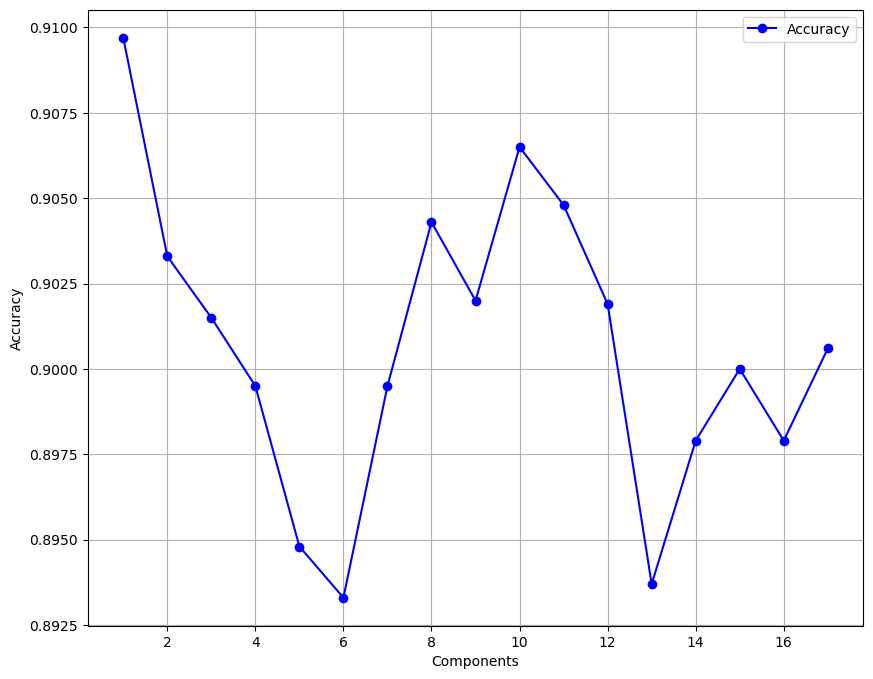
\includegraphics[width=\linewidth]{gmm-accuracy.png}
        \caption{Accuracy}
      \end{subfigure}
      
      \vspace{1em}
      
      \begin{subfigure}{\linewidth}
        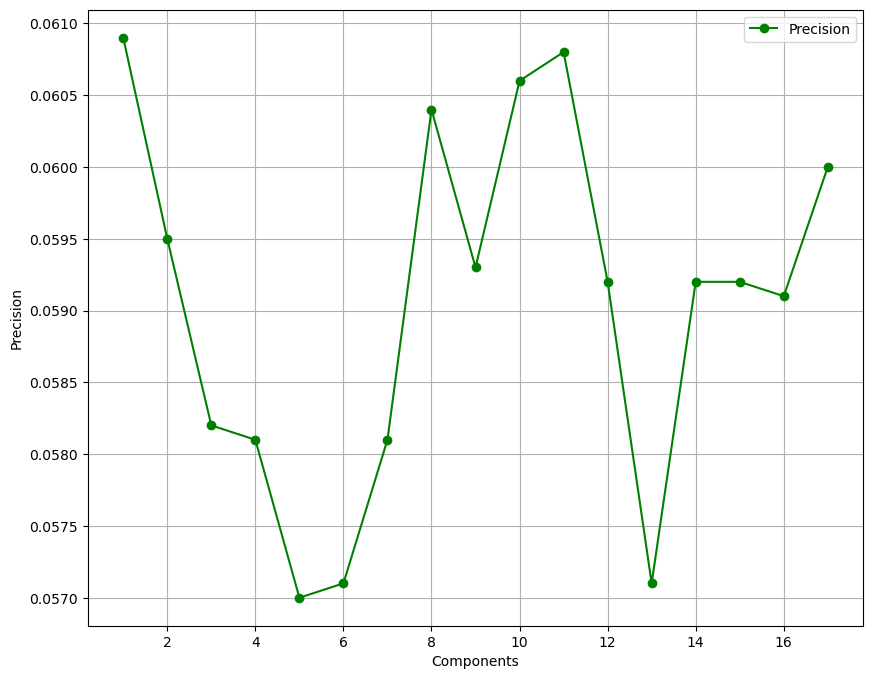
\includegraphics[width=\linewidth]{gmm-precision.png}
        \caption{Precision}
      \end{subfigure}
    \end{minipage}%
    \begin{minipage}{0.5\textwidth}
      \begin{subfigure}{\linewidth}
        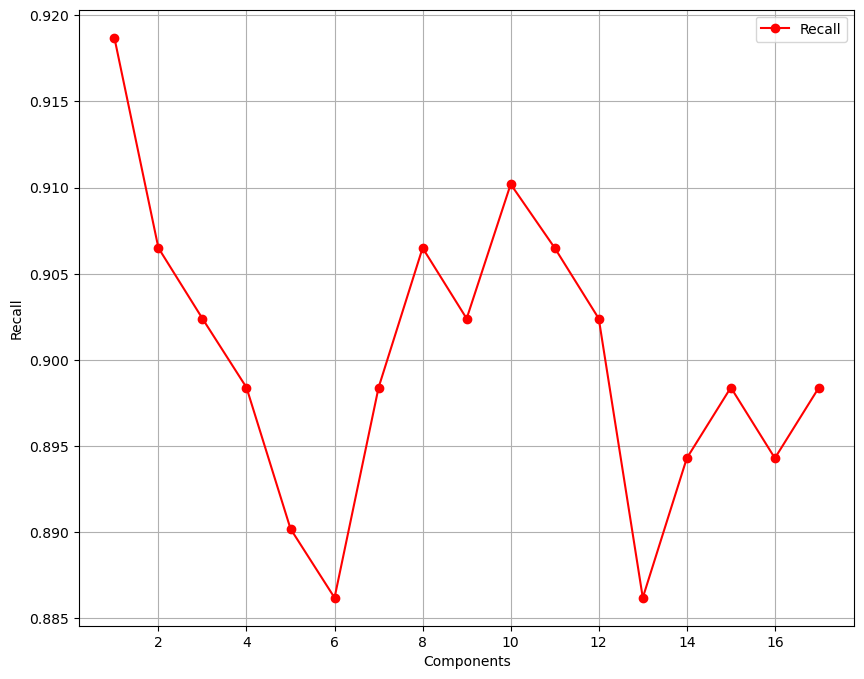
\includegraphics[width=\linewidth]{gmm-recall.png}
        \caption{Recall}
      \end{subfigure}
    \end{minipage}
    
    \caption{Evoluţia valorilor metricilor de performanţa pentru GMM}
\end{figure}
  

\section{Kernel Density Estimation}

\begin{table}[htb]
    \centering
    \begin{tabularx}{\textwidth}{
        |X
        |X
        |X
        |X|
    }
    \hline
    {Bandwidth} & {Accuracy} & {Precision} & {Recall} \\
    \hline
    \rowcolor{gray!20} 0.01 & 0.066 & 0.002 & 1.000 \\
    0.1 & 0.155 & 0.002 & 1.000 \\
    \rowcolor{gray!20} 0.2 & 0.251 & 0.002 & 1.000 \\
    0.5 & 0.489 & 0.003 & 1.000 \\
    \rowcolor{gray!20} 1.0 & 0.845 & 0.011 & 0.959 \\
    5.0 & 0.900 & 0.016 & 0.946 \\
    \rowcolor{gray!20} 10.0 & 0.900 & 0.016 & 0.946 \\
    \hline
    \end{tabularx}
    \caption{Performanța creşte cu valoare lăţimii de bandă}
\end{table}

Folosim \textbf{kernelul Gaussian}.

Se observă ca după $5.0$, valoarea lăţimii de banda nu mai aduce îmbunătăţiri 
semnificative. Chiar dacă recall se degradează puţin, nu vom alege niciuna din 
valorile mai mici decât $1.0$, întrucât acurateţea este multe prea mică pentru 
practicalitate. Daca semnalăm aproape toate observaţiile ca fiind anomalii, atunci 
algoritmul devine inutil.

Alegem \textbf{lăţimea de bandă} $bandwidth=5.0$ pentru modelul final, aceasta fiind cea mai mică valoare 
care aduce o performanţă decentă. O valoare prea mare a lăţimii de banda duce 
la o netezire excesivă a particularităţilor distribuţiei.


\begin{figure}[htbp]
    \begin{minipage}{0.5\textwidth}
      \begin{subfigure}{\linewidth}
        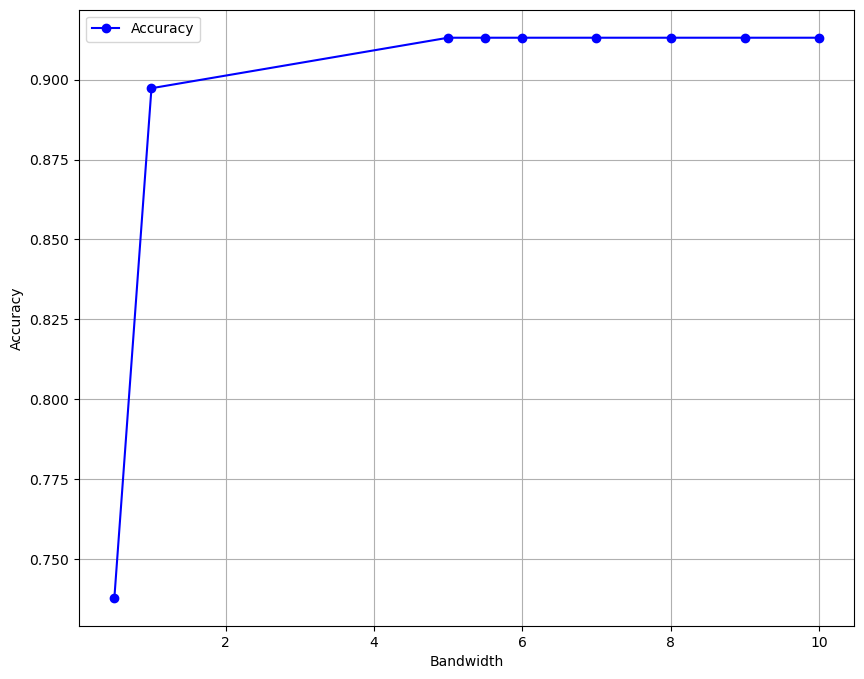
\includegraphics[width=\linewidth]{kde-accuracy.png}
        \caption{Accuracy}
      \end{subfigure}
      
      \vspace{1em}
      
      \begin{subfigure}{\linewidth}
        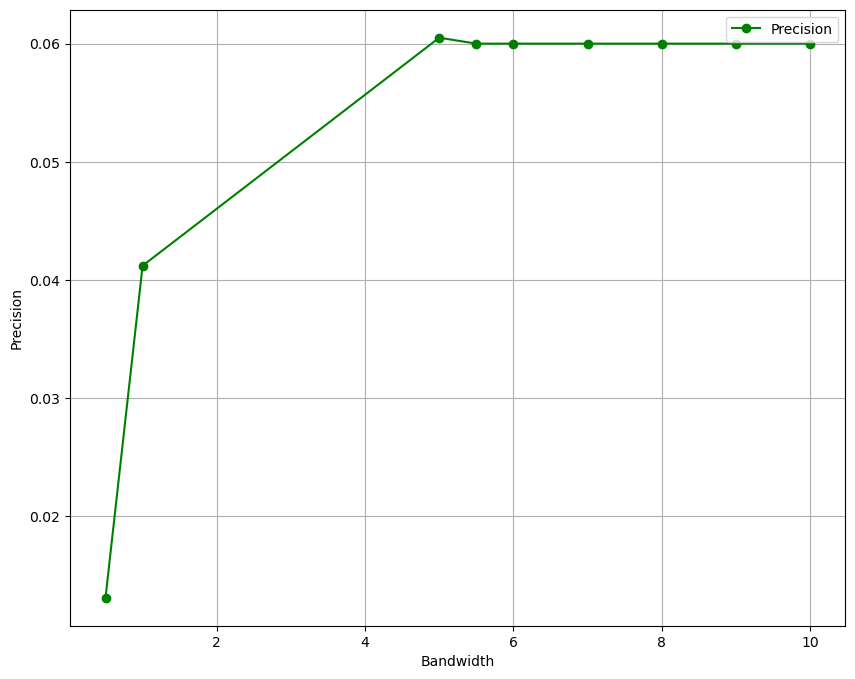
\includegraphics[width=\linewidth]{kde-precision.png}
        \caption{Precision}
      \end{subfigure}
    \end{minipage}%
    \begin{minipage}{0.5\textwidth}
      \begin{subfigure}{\linewidth}
        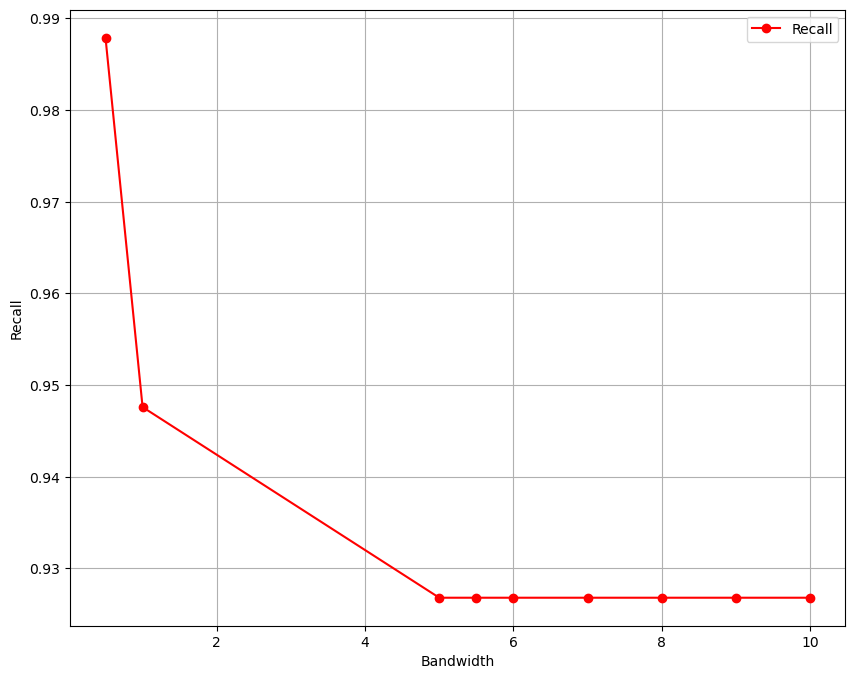
\includegraphics[width=\linewidth]{kde-recall.png}
        \caption{Recall}
      \end{subfigure}
    \end{minipage}
    
    \caption{Evoluţia valorilor metricilor de performanţa pentru KDE}
\end{figure}
